\pagelayout{margin} % Restore margins

\setchapterstyle{kao}
\setchapterpreamble[u]{\margintoc}
\chapter{Electromobility and Climate Change}

This chapter explores the motivations behind the transition to electric mobility, examining the environmental causes driving this shift, the evolution of electric vehicles, regulatory frameworks accelerating adoption, and the critical infrastructure challenges that must be addressed to enable widespread electrification of transportation. One of the identified challenges, which is demand for chargers will be introduced. It will be the main topic of this thesis and our focus on predicting it based on existing data for new potential charger locations to aid the decision making process.


\section{Climate change}

Climate change represents one of the most pressing global challenges of our time, with transportation being a significant contributor to greenhouse gas emissions. The burning of fossil fuels is the primary driver of anthropogenic climate change, with transportation accounting for approximately 24\% of direct CO\textsubscript{2} emissions from fuel combustion globally \cite{quadrelliEnergyClimateChallenge2007}.

The environmental impact of ICE vehicles extends beyond carbon dioxide emissions. These vehicles also produce other polutants. Which have negative health outcomes like increased mortality (about 3\% of mortality in Europe \cite{kunzliPublichealthImpactOutdoor2000}), asthma attacks, higher cardiovascular hospital admissions, higher repiratory hospital admissions \cite{kunzliHealthCostsDue1999}.

\begin{figure}[h]
    \centering
    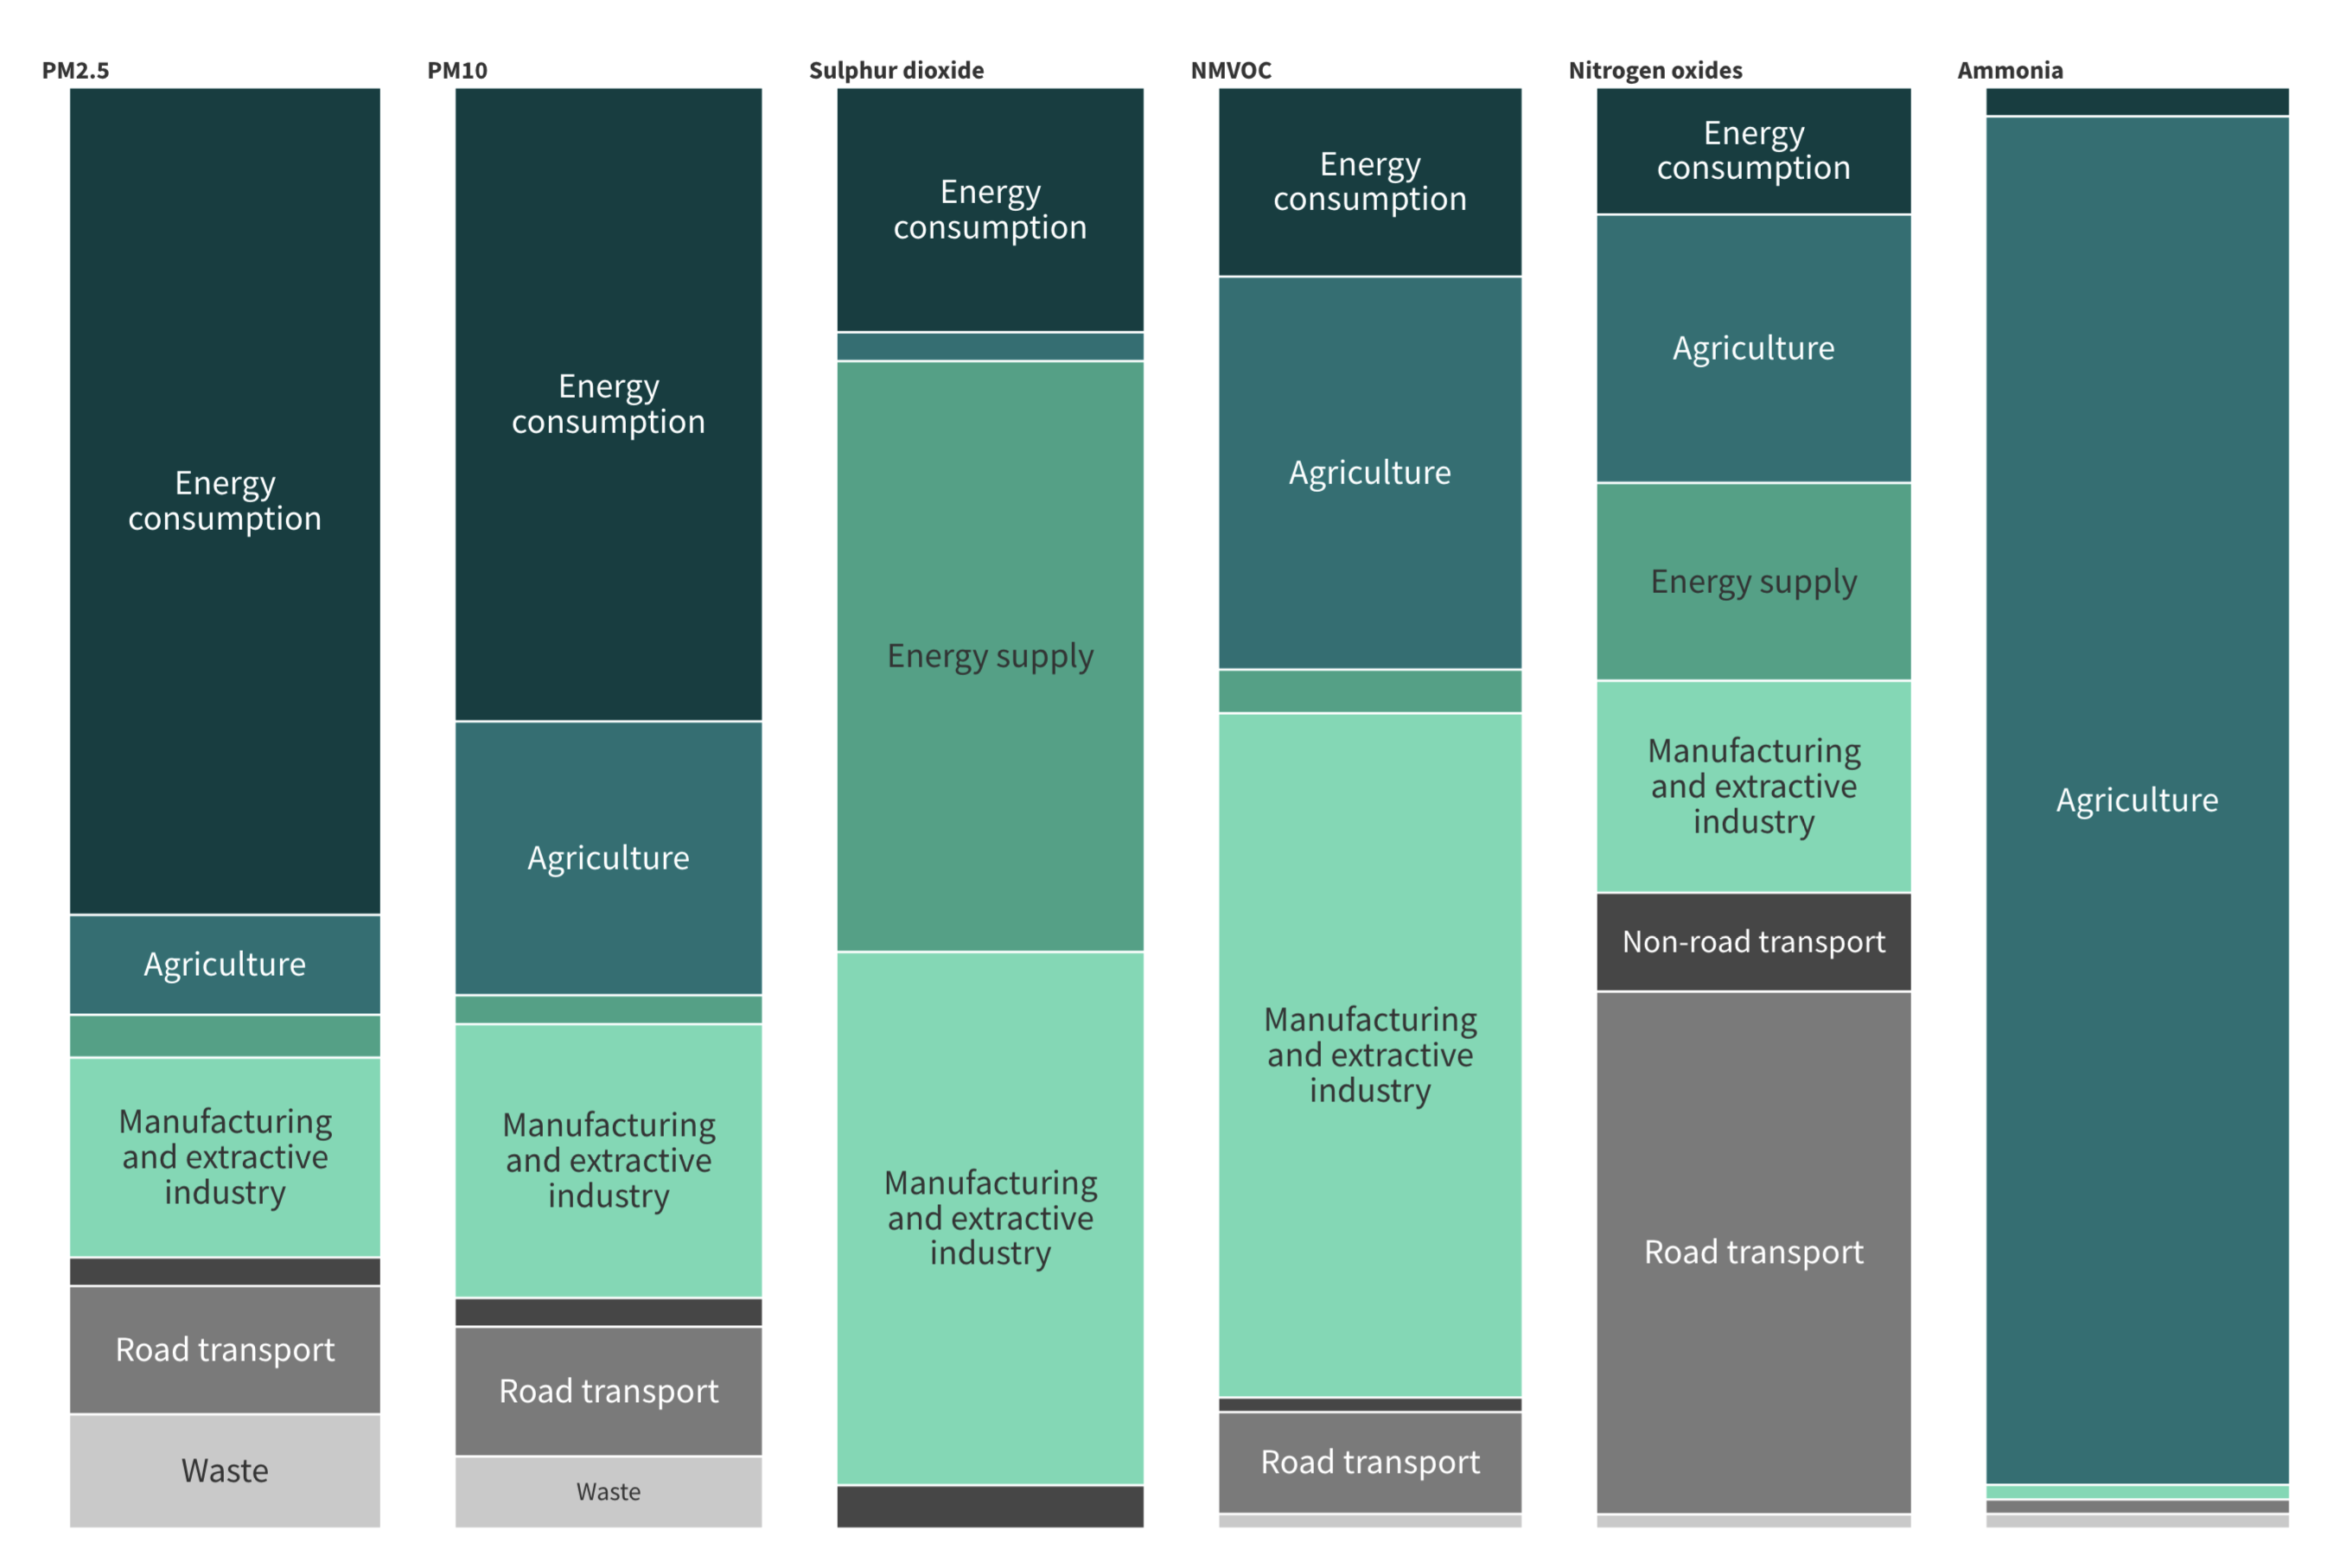
\includegraphics{introduction/polution_source.png}
    \label{fig:polution_source}
    \caption{Share of EU emissions in 2020. PM2.5 = fine particulate matter; PM10 = particulate matter; Energy consumption = residential, commercial and institutional energy consumption; NMVOC = non-methane volatile organic compounds. Source \cite{ContributionsEU27Emissions2022}}
\end{figure}

While the scientific consensus on anthropogenic climate change is robust, it is worth acknowledging that the transition to electric mobility is not without controversy. The manufacturing process of \acrlong{EV} has higher negative enviromental impact compared to \acrlong{ICE} due to battery manufacturing. But they have a chance to mitigate this over their lifetime use if the share of generated energy for their use comes from sustainable sources. Combined with remanufacturing and recycling of old batteries. \sidecite{xiaReviewLifeCycle2022a}

\section{Electric vehicles}

The history of electric vehicles (EVs) is marked by a parallel development alongside internal combustion engine vehicles, rather than being a purely modern innovation. In fact, electric vehicles were among the first automobiles developed in the late 19th century, with inventors like Gustav Trouvé creating electric cars as early as 1881 \sidecite{wakefield1998history}. During the early automotive era, electric vehicles competed directly with steam and gasoline powered vehicles. And even had dominance in early 20th century (An electric vehicle taxi existed for a short period of time in 1987 London \sidecite{SurprisinglyOldStory2012}).

However, the limitations of early battery technology—particularly in terms of energy density, range, and recharging infrastructure—combined with the discovery of abundant petroleum reserves and the introduction of the electric starter for gasoline engines, led to the dominance of ICE vehicles throughout most of the 20th century . And use of electric engines in transportation remained in city trams and subways.

The modern resurgence of electric vehicles began in the late 1990s and early 2000s, driven by advances in lithium-ion battery technology, growing environmental concerns. The introduction of hybrid vehicles like the Toyota Prius served as a transitional technology, familiarizing consumers with electric drivetrains while alleviating range anxiety through the backup of a gasoline engine. The launch of the Tesla Roadster in 2008 demonstrated that electric vehicles could offer performance comparable to or exceeding that of high-end sports cars, challenging perceptions that EVs were inherently limited in capability \sidecite{ElectricVehicleFuture}.

Today's electric vehicles have largely overcome many of the historical limitations that hindered their adoption. Modern EVs offer ranges exceeding 300-400 kilometers on a single charge, with high-end models approaching 600 kilometers. Fast-charging infrastructure has expanded significantly, enabling long-distance travel with reasonable charging stops. The total cost of ownership for EVs has become increasingly competitive with ICE vehicles due to lower operating and maintenance costs, despite higher initial purchase prices. A gap that continues to narrow as battery costs decline and economies of scale improve (see Figure \ref{fig:ev-sales}).


\begin{figure}[h]
    \centering
    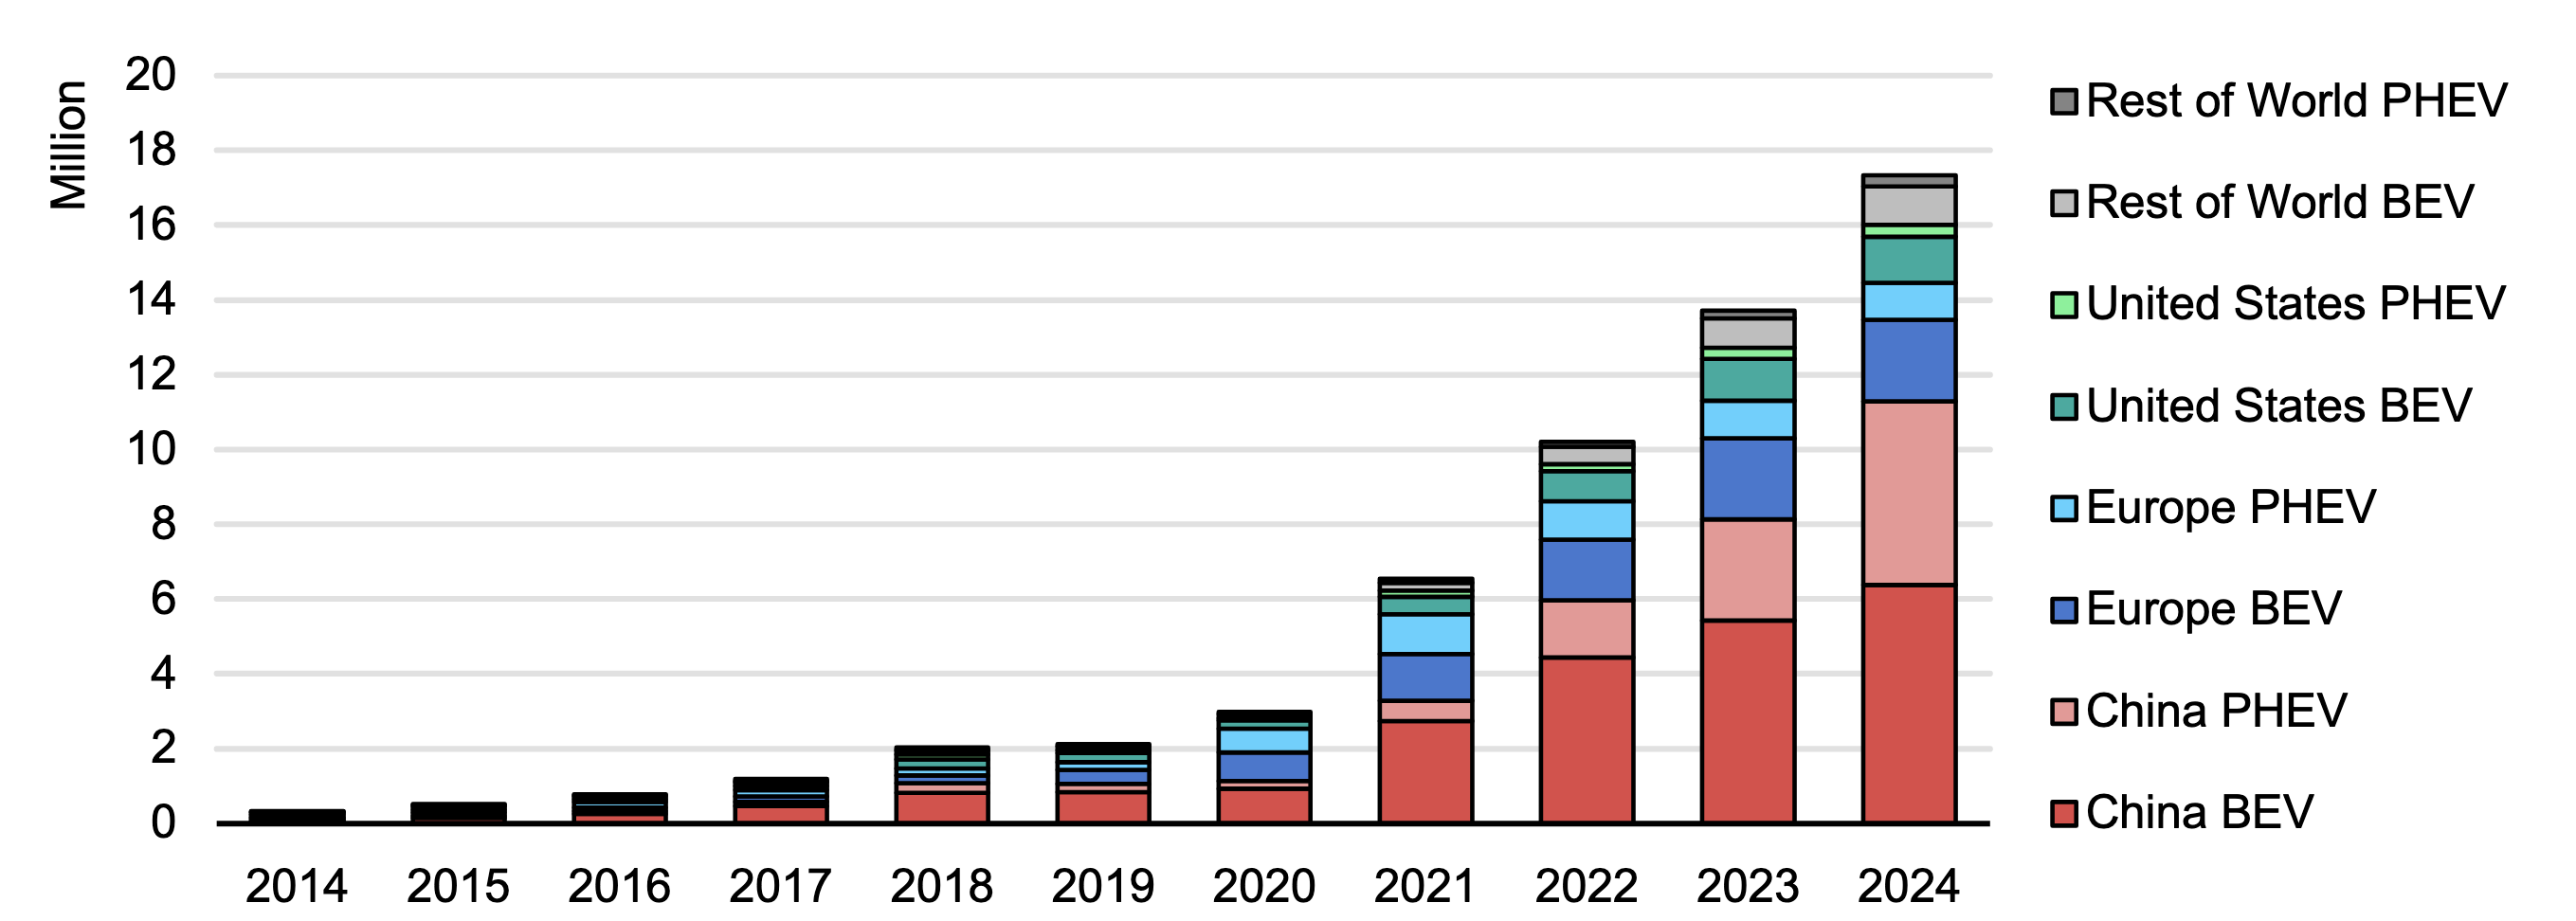
\includegraphics{introduction/ev_sales_rise.png}
    \caption{Global electric car sales, 2014-2024. Source: IEA analysis based on country submissions, ACEA, EAFO, EV Volumes and Marklines \cite{IEA2024}}
    \label{fig:ev-sales}
\end{figure}


The environmental benefits of electric vehicles are substantial, particularly when powered by low-carbon electricity sources. Even when accounting for the current global electricity mix, which still includes significant fossil fuel generation, EVs typically produce lower lifecycle greenhouse gas emissions than comparable ICE vehicles. As electricity grids continue to decarbonize, this advantage will only increase (see Figure \ref{fig:co2_predictions_czechia}). Additionally, the shift of emissions from millions of individual tailpipes to centralized power plants offers significant air quality benefits in urban areas and creates opportunities for more efficient pollution control.

\begin{figure}[h]
    \centering
    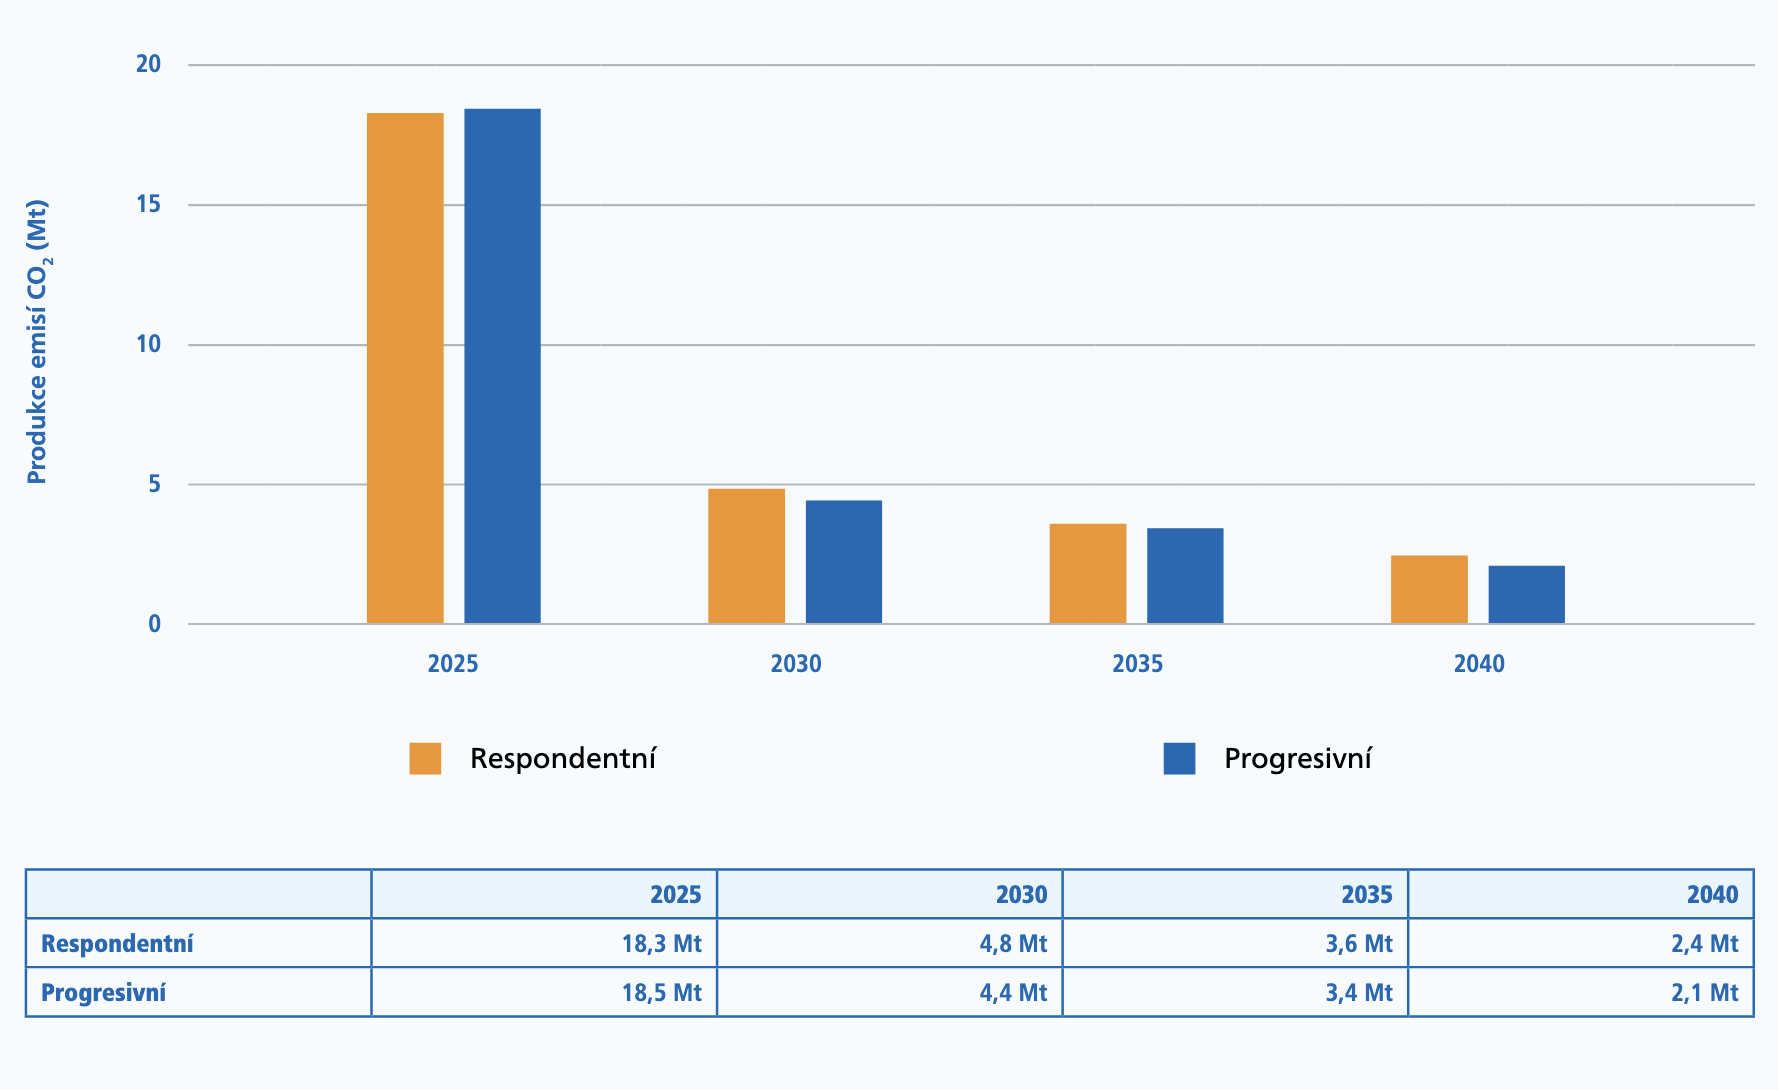
\includegraphics{introduction/co2_predictions.png}
    \caption{CO\textsubscript{2} emission  from electricity production prediction for Czechia for selected years \cite{CEPS}}
    \label{fig:co2_predictions_czechia}
\end{figure}

However, the transition to electric mobility faces many of the same infrastructure challenges that the early automobile industry encountered. Just as the widespread adoption of ICE vehicles required the development of a comprehensive network of gas stations, repair facilities, and roads, the EV revolution depends on the deployment of charging infrastructure, grid upgrades, and maintenance expertise. These parallels suggest that while the challenges are significant, they are not unprecedented and can be overcome through coordinated investment and policy support.

\section{EU mandate}



The European Union has established regulatory framework to accelerate the transition to electric mobility as part of its broader climate strategy. The cornerstone of this approach is Regulation (EU) 2019/631 \sidecite{RegulationEU20192019}, which sets CO\textsubscript{2} emission performance standards for new passenger cars and light commercial vehicles. This regulation is part of "Fit for 55" package proposed in July 2021 and subsequently adopted, which aims to reduce net greenhouse gas emissions by at least 55\% by 2030 compared to 1990 levels \sidecite{CasovaOsaZelena}\sidecite{CoJeFit}.

The most transformative element of this regulatory framework is the mandate that effectively prohibits the sale of new internal combustion engine vehicles in the EU from 2035 onward. Specifically, the regulation requires a 100\% reduction in CO\textsubscript{2} emissions from new cars and vans by 2035 compared to 2021 levels, which in practice means that only zero-emission vehicles—battery electric or hydrogen fuel cell—can be sold as new vehicles after this date. This represents a clear and unambiguous signal to the automotive industry, infrastructure developers, and consumers about the direction of transportation policy in Europe.

The EU's approach includes intermediate targets to ensure a gradual transition: a 55\% reduction in car emissions and a 50\% reduction in van emissions by 2030 compared to 2021 levels. These targets are accompanied by incentive mechanisms for zero- and low-emission vehicles, penalties for manufacturers that exceed fleet-wide emission targets, and provisions for reviewing the effectiveness of the regulation.

This regulatory certainty has already catalyzed significant investment in electric vehicle production and charging infrastructure across Europe. Major automotive manufacturers have announced accelerated timelines for electrifying their fleets, with many planning to phase out ICE vehicle production well before the 2035 deadline. The mandate has also spurred innovation in battery technology, charging solutions, and vehicle design as companies compete to position themselves advantageously in the emerging electric mobility ecosystem.

By establishing a definitive end date for new ICE vehicle sales, the EU has moved beyond incremental improvements to fossil fuel efficiency and committed to a fundamental technological transition in personal transportation.

\begin{figure}
    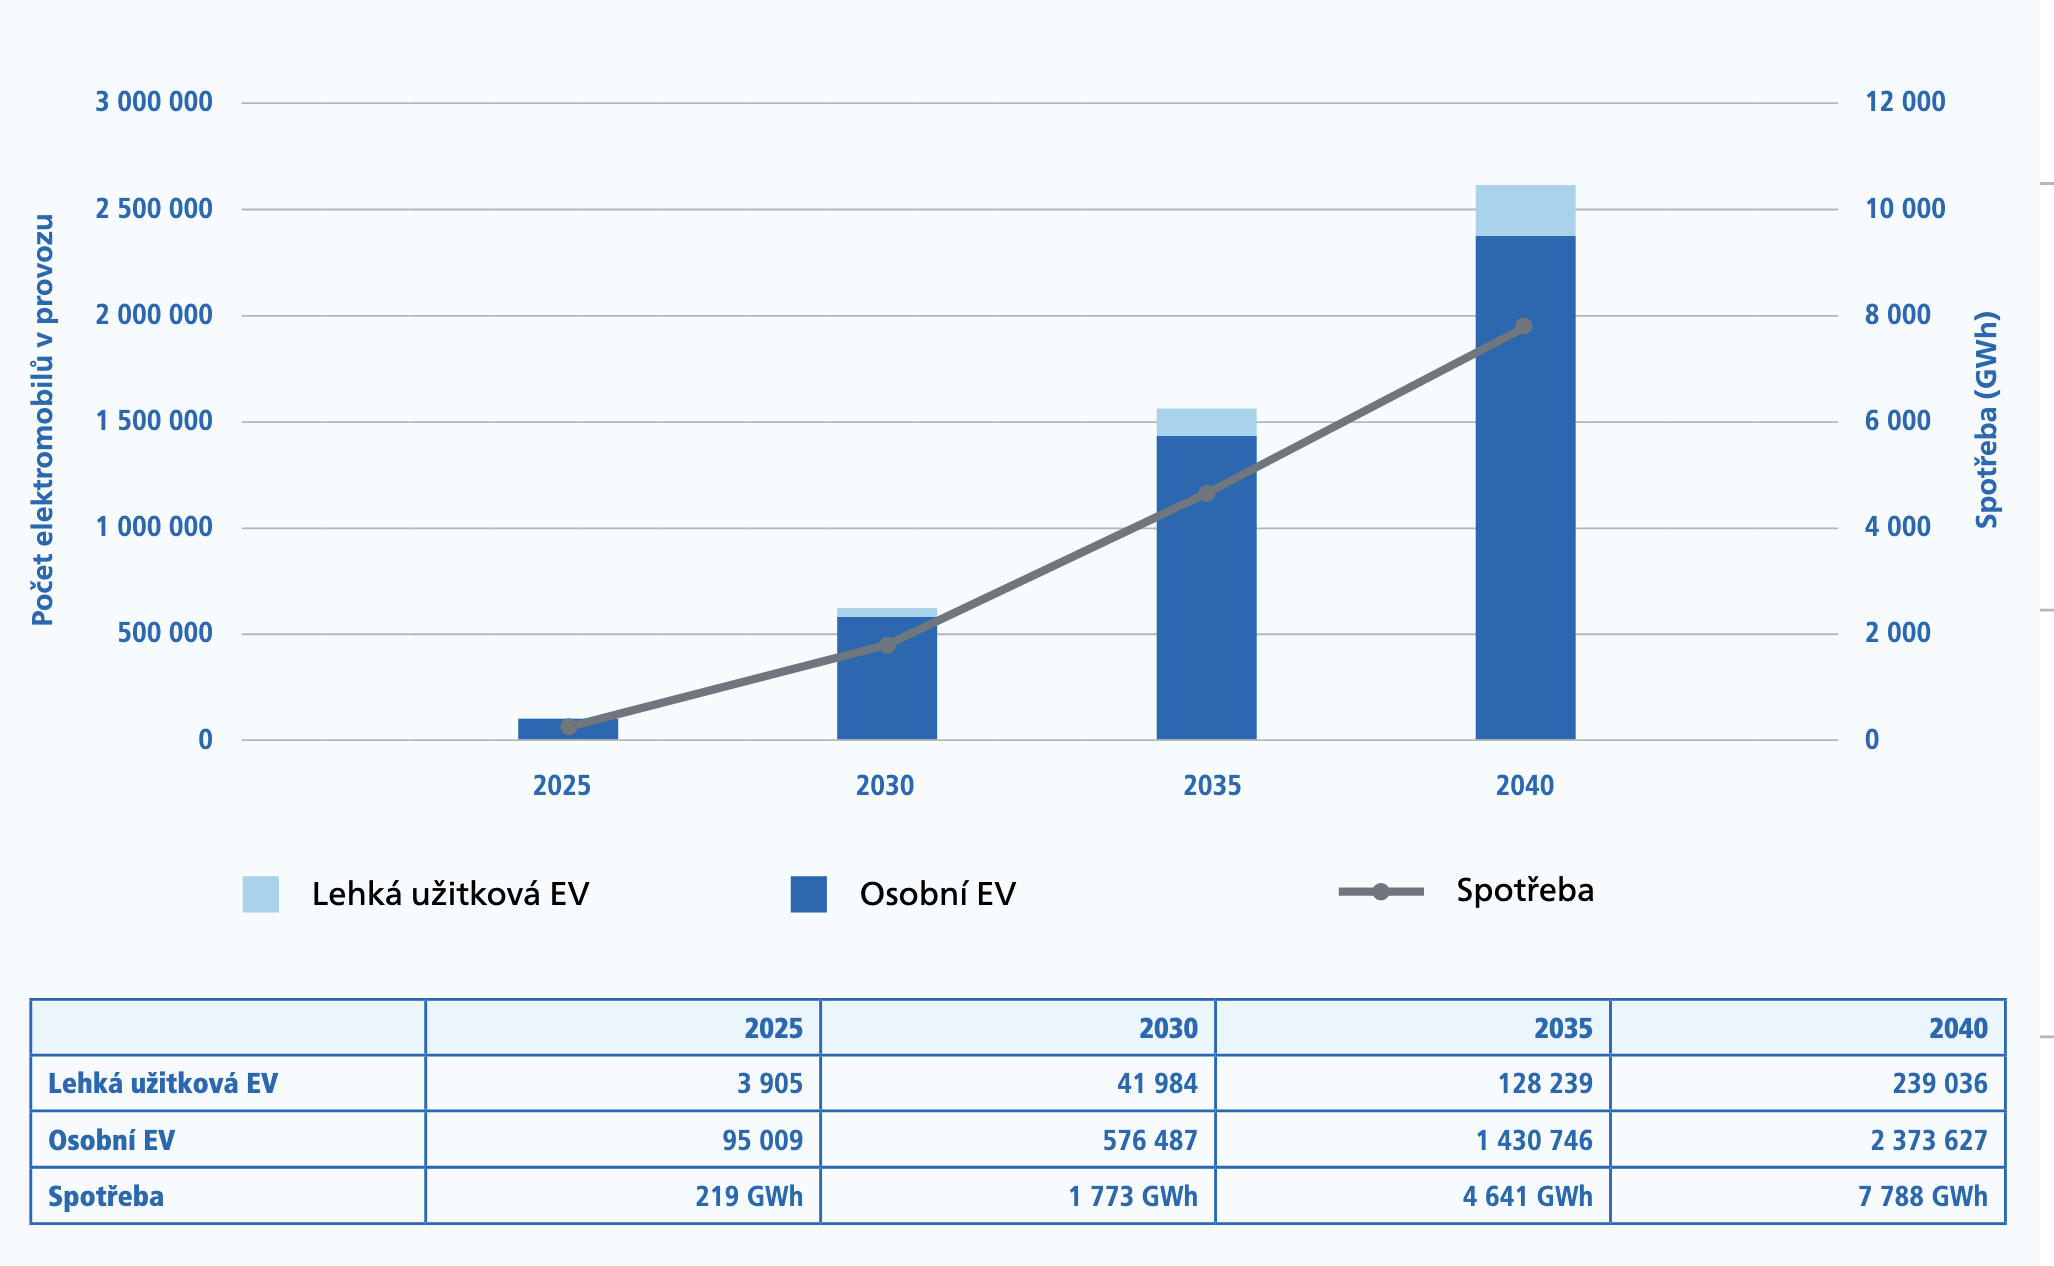
\includegraphics{introduction/ev_prediction_czechia.png}
    \caption{Prediction on number of EVs in Czechia taking into account the (EU) 2019/631 regulation }
\end{figure}

\section{Electric Vehicle Chargers}

Due to high urban density in Prague. Especially in the city center which mostly consist of apartment buildings. Street parking is the dominant type of parking here. Those parking locations do not have easy access to \acrlong{EV} charging and they require construction as well as having the power source somewhere (underground). Opposed to single family housing where high number of parking spots is located on the houses private land. Where there is higher accessibility to private electric charger. Where the simplest solution can be an electrical outlet.

Modern EV charging infrastructure can be categorized by power output, which directly affects charging speed \sidecite{Regulation20231804}:

\begin{itemize}
    \item \textbf{Category 1 (AC):}
          \begin{itemize}
              \item \textbf{Slow AC charging:} Utilizing standard household outlets (P < 7.4 kW). While inadequate as a primary charging solution for most users, they serve as emergency options or for overnight charging in residential settings.

              \item \textbf{Medium-speed AC charging:} Operating at 7.4-22 kW, these chargers can fully replenish most EV batteries in 4-8 hours.

              \item \textbf{Fast AC charging:} Operating at > 22 kW.
          \end{itemize}

    \item \textbf{Category 2 (DC):}
          \begin{itemize}
              \item \textbf{Slow DC charging:} Less than 50 kW.

              \item \textbf{Fast DC charging:} 50-150 kW.

              \item \textbf{Ultra-fast DC charging:} 150-350 kW and above.
          \end{itemize}
\end{itemize}

DC fast charging stations can provide an 80\% charge in 20-40 minutes for compatible vehicles. They are strategically deployed along major travel corridors and in urban centers to enable long-distance travel and quick top-ups for those without home charging access.

The installation costs vary based on charger type. A significant challenge is managing grid load, particularly during peak demand periods such as after-work hours. This has led to the development of smart charging systems with dynamic pricing. Chargers can also be installed in public lighting lamps as a cost-effective solution.

The technical challenges of charging infrastructure placement extend beyond the charging equipment itself to include grid integration considerations. High-power charging stations can place significant demands on local distribution networks, potentially requiring costly grid upgrades or reinforcement. Strategic placement that aligns with existing grid capacity can substantially reduce deployment costs and timelines.

Data-driven approaches to infrastructure planning incorporate multiple data sources including traffic patterns, demographics, points of interest, existing infrastructure utilization, grid capacity, and temporal mobility patterns. By integrating these diverse datasets, planners can develop models that predict charging demand with high temporal and spatial resolution, enabling more efficient infrastructure deployment that maximizes utilization while minimizing costs.

\section{Goals of the thesis}

This thesis explores the challenge of predicting electric vehicle charging demand in Prague through data analysis and machine learning approaches. Working with data provided by PREdistribuce, this research investigates whether spatial and temporal features can effectively predict charging patterns. The specific objectives addressed in this thesis are:

\begin{itemize}
    \item To examine the current state of electromobility and climate change, establishing the context for the growing importance of charging infrastructure planning

    \item To analyze charging session data from PREdistribuce's network of public charging stations in Prague, transforming raw session data into hourly power consumption patterns

    \item To integrate publicly available spatial data sources, including Basic Settlement Units (ZSJ) demographics and OpenStreetMap points of interest, with charging data to create a comprehensive feature set

    \item To develop a neural network model with latent profiles that attempts to capture underlying patterns in charging behavior while maintaining interpretability

    \item To evaluate the model's performance against baseline approaches (average model, linear regression, XGBoost) using various error metrics

    \item To analyze the learned latent profiles to determine if meaningful charging patterns could be extracted despite the model's overall performance limitations

    \item To identify data limitations and suggest potential improvements for future research in charging demand prediction
\end{itemize}

This research represents an initial exploration into charging demand prediction in the context of Prague, acknowledging the challenges of limited data availability and quality. While the predictive performance did not exceed baseline models, the methodological approach and analysis of limitations provide valuable insights for future research directions in this field.
